\documentclass[oneside]{book}
\usepackage{graphicx}
\graphicspath{{img/}}
%\usepackage{fancyvrb}


\usepackage{color}
\usepackage{fourier-orns}
\usepackage{lettrine}
\usepackage[hidelinks]{hyperref}
\usepackage{float}
\usepackage{wallpaper}

\input Acorn.fd
\newcommand*\initfamily{\usefont{U}{Acorn}{xl}{n}}
\definecolor{darkgreen}{RGB}{0,80,0}
\definecolor{darkgray}{RGB}{33, 33, 33}
\newcommand{\ornamento}{\vspace{2em}\noindent \textcolor{darkgreen}{\hrulefill~ \raisebox{-2.5pt}[10pt][10pt]{\leafright \decofourleft \decothreeleft  \aldineright \decotwo \floweroneleft \decoone   \floweroneright \decotwo \aldineleft\decothreeright \decofourright \leafleft} ~  \hrulefill \\ \vspace{2em}}}




\begin{document}
\clearpage
 \TileWallPaper{614pt}{800pt}{scroll.jpg}

%% temporary titles
% command to provide stretchy vertical space in proportion
\newcommand\nbvspace[1][3]{\vspace*{\stretch{#1}}}
% allow some slack to avoid under/overfull boxes
\newcommand\nbstretchyspace{\spaceskip0.5em plus 0.25em minus 0.25em}
% To improve spacing on titlepages
\newcommand{\nbtitlestretch}{\spaceskip0.6em}
\pagestyle{empty}

\begin{center}
  \bfseries
  %\nbvspace[1]
  \Large
  {\nbtitlestretch\textcolor{darkgreen}{\lettrine[lines=3]{\initfamily{T}}
  {HIS IS FAIRY'S ALBUM}}}

\nbvspace[1]
\normalsize

\nbvspace[1]
\textcolor{darkgray}{
  \small READING MATERIAL FOR THE\\
  \Large ESL IN ACTION COURSE\\[0.5em]
  \footnotesize READER 1}
\nbvspace[2]

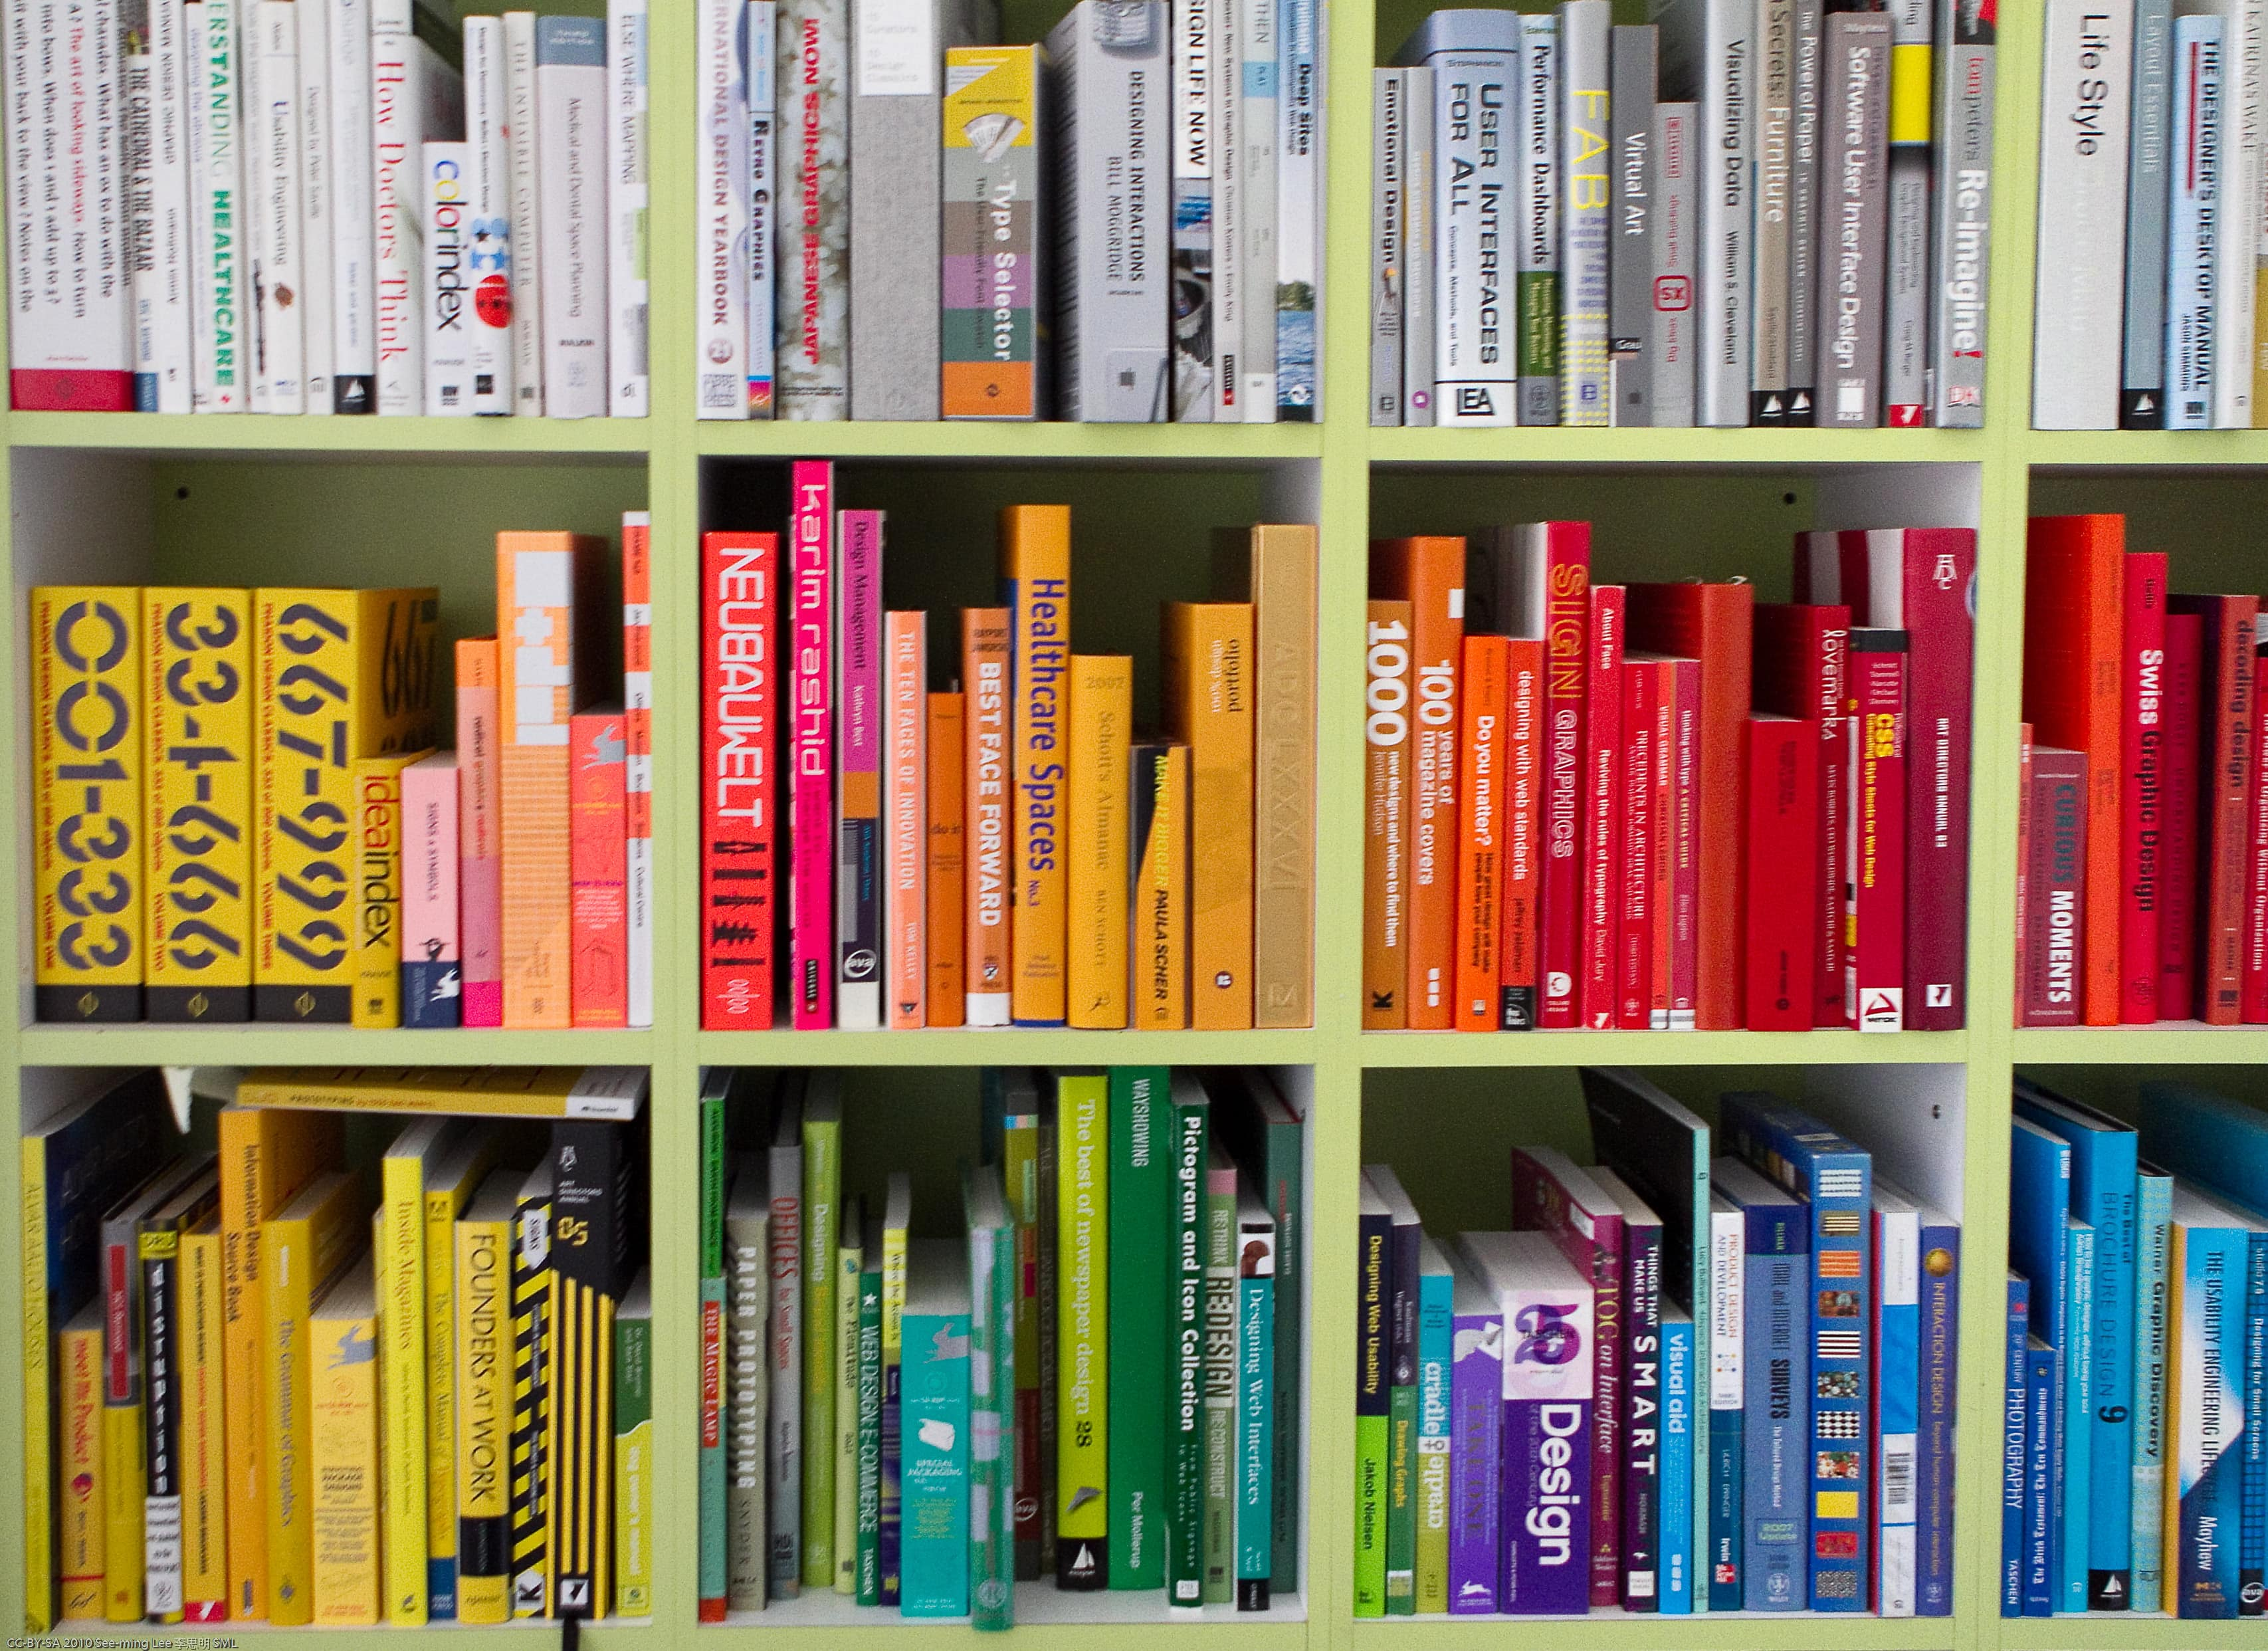
\includegraphics[width=4.5in]{books.jpg}
\nbvspace[3]
\normalsize

\ornamento
\large
\textcolor{darkgray}{
  PUBLISHED BY LIVE AFTER 60 \\
  \href{https://www.liveafter60.com}{www.liveafter60.com}}
\nbvspace[1]
\end{center}

\newpage
\frontmatter
\vspace*{15ex}
\begin{center}
  Copyright \copyright\ 2020 Live After 60.\\
  Released under the \\
  Creative Commons Attribution-ShareAlike 3.0 Unported License.\\
  \href{https://creativecommons.org/licenses/by-sa/3.0/}{
    https://creativecommons.org/licenses/by-sa/3.0/}
  \begin{figure}[H]
    \centering
    
\includegraphics[scale=0.8]{cc-by-sa}
  \end{figure}
  Adapted from ``Fairy's Album With Rhymes of Fairyland''.\\ 
  Available in the Public Domain through Project Gutenberg.\\
  \href{https://www.gutenberg.org}{https://www.gutenberg.org}\\
  \bigskip
  Audio adapted from Librivox.\\
  \href{https://librivox.org}{https://librivox.org}\\
  \bigskip
  Cover image \copyright\ CC-BY-SA See-ming Lee.\\
  \href{https://www.flickr.com/photos/seeminglee/4556156477/sizes/l/}{https://www.flickr.com/photos/seeminglee/4556156477/sizes/l/}\\
  \bigskip
  Reviewed by Prof. Dr. Jnanabrata Sil.\\
  \href{drjsil@gmail.com}{drjsil@gmail.com} \\
  \bigskip
  Typeset in \LaTeX\ based on the motif suggested by @Fran. \\
  \href{https://tex.stackexchange.com}{https://tex.stackexchange.com} \\
  \bigskip
  Edited and published by Live After 60 as part of its ``ESL in Action''
	course.\\
  \href{http://www.liveafter60.com}{www.liveafter60.com}
\end{center}
\vspace*{15ex}

\end{document}
